\documentclass[conference]{IEEEtran}
\title{Location-based and Communicative Game Platform Improving Learning
Toward Stage passing}
\date{June 8, 2014}
\author{Masoumeh Seydi\\ Department of Computer Science\\
       Konstanz University, Germany}

\usepackage{graphicx}
\begin{document}
\maketitle

\section{Introduction}
Through the state of the art concepts in serious gaming~\cite{sergame1,sergame2}, 
there are noticeable efforts to use it for the learning purposes~\cite{sergame3} as well.
\footnote{We mean the general definition of the serious games as 
usage of games to simulate the serious situations.}
No one has doubts that the main element of each game is 
the scenario that players follow.
Although there is a long tradition in generating a game
for a specific purpose and specific scenario, 
there is still room for research 
to find a more general purpose framework for various scenarios.

In this proposal, our aim is to generate a game platform 
which is flexible to adapt to new different situations coming
from various ways of adventure scenarios. 
To achieve this goal, we combine the following elements:
\begin{itemize}
\item Learning based on the location-based games like~\cite{rexplorer} or in 
a large scale~\cite{scal-loc-g}.
\item The ability of the sensors in mobile phones like the ones explained in~\cite{sensors}.
\item Adapting the scenarios and generating the breakpoints
\item Attachment of game elements to each breakpoint (for a try in this direction 
look at \cite{totem})
\end{itemize}


Each story has some basic components such as characters, the main different stages which leads to the end, and happenings. In our game which is based on a story, the stages can include a location, sound or image hints, contacts, and messages, and augmented reality as a goal which should be met. The players must reach the goals in each stage and can communicate with each other by providing online of offline sound, image, and text messages either. It means that for each point in a process the players can either contact each other directly or save a message. Then, the others could read or hear it when they want. The message could be specified to a location. In this case, the messages will be shown as a hint in that location when the players arrive to that location. These messages can be hints or information about the path or the goal they are following.

\section{Scenario}
\cite{scenario}

This needs a specific research over both 


A research is also needed regarding the human interaction and communication
together and with the device, like \cite{behavior} and \cite{facial-vocal}.

\cite{scenario-adapt}
\cite{scenario-repurposing}


\cite{scenario-gen}
\cite{l-system}

%-----------------------------------------------------------------
\begin{figure}
 \centering
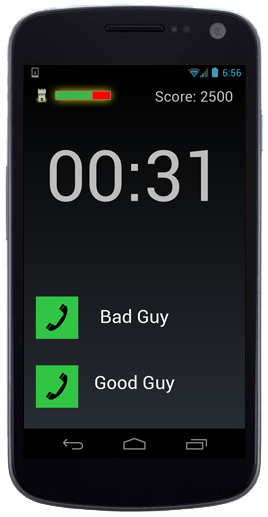
\includegraphics[width=0.14\textwidth]{kar}
\caption{The Starting page of mobile (Prototype}
\label{diagram}
\end{figure}
%-----------------------------------------------------------------


\bibliographystyle{unsrt}
\bibliography{refs}
\end{document}
